\subsection{Begriff}
\begin{itemize}
\item Polarisation ist festgelegt durch die Schwingungsebene der elektrischen Feldstärke des Lichtes.
\item Natürliches Licht ist unpolarisiert, d.h. es enthält Licht aller Polarisationsrichtungen, also in allen Schwingungsebenen.
\end{itemize}

\subsection{Polarisationsfilter}
\begin{itemize}
\item In eine einzige Richtung polarisiertes Licht wird zu 100\% durchgelassen, wenn sicher der Filter in Transmissionsrichtung befindet. Bei 90\degree zur Trasmissionsrichtung wird es zu 100\% abgeschirmt.
\item Malus'sches Gesetz: Intensität $I_1$ vor Filter; $I_2$ nach Filter
\item $I_2 = I_1 \cdot cos^2(\Theta)$
\end{itemize}

\subsection{Brewster-Winkel}
\begin{itemize}
\item Licht kann auch durch Reflexion polarisiert werden. Wenn das Licht im Brewter-Winkel auftrifft, wird der reflektierte Strahl vollständig polarisiert.
(E-Feld steht dann parallel zur Reflexionsebene)
\item Bedingung für vollständige Polarisation: Winkel zwischen reflektiertem und gebrochenem Strahl muss gleich 90\degree sein.
\item $\beta = 90\degree - \alpha_B$
\item $\frac{\sin{\alpha_B}}{\sin{90\degree - \alpha}} = \frac{n_2}{n_1}$ \tabto{4cm}; siehe Brechungsgesetz
\item $\frac{\sin{\alpha_B}}{\cos{\alpha_B}} = \tan{\alpha_B} = n_2$ \tabto{4cm}; $n_1$ ist 1 für Luft bzw. Vakuum

\begin{figure}[h!]
\centering 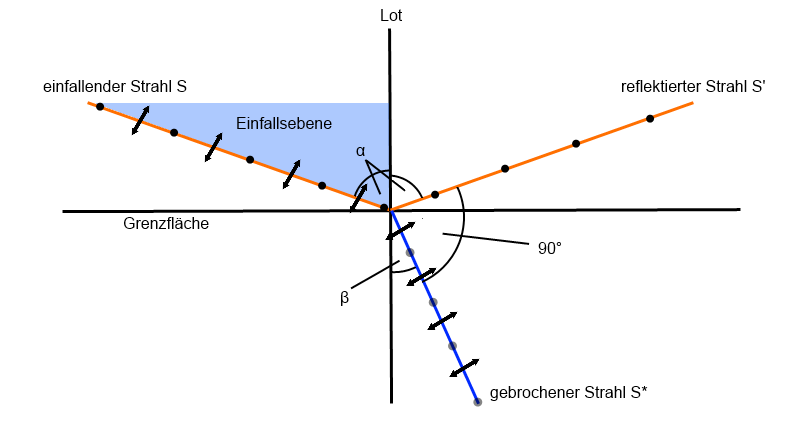
\includegraphics[width=0.8\textwidth]{brewster_winkel}
\caption{Abbildung von \url{http://phy.wdfiles.com/local--files/polarisiertes-licht-c-j/Brewster\%20Winkel\%204.png}}
\end{figure}

\end{itemize}